%Estandarización de los títulos, identación e entrelineado
\titleformat{\chapter}[display]
  {\normalfont\bfseries}{}{0pt}{\Huge}
\titlespacing{\chapter}{0pt}{0cm}{2pt}
\titleformat{\section}[display]
  {\normalfont\bfseries}{}{0pt}{\Large}
\titlespacing{\section}{0pt}{0cm}{1pt}

% Escrito
\chapter{Introducción}
\lipsum[1] %TEXTO

\section{Tema 1} %PRIMER TEMA O CAPITULO DE LA INTRODUCCIÓN
\lipsum[2-3] %TEXTO

%EJEMPLO DE TABLA
\begin{table}
	\centering
	\caption{Tabla 1}
	\label{tabla:1}
	\begin{tabular}{|c|c|c|r|}
		\hline
		\textbf{Gatos} & \textbf{Gatos Blancos} & \textbf{Gatos Negros} & \textbf{Proporcion} \\\hline
		\textbf{Gatitos} & $2.354\times10^4$ &  $17,482$ & $1.34652$\\
		\textbf{Gatetes} & $52,334$ & $3.634\times10^3$ & $14.40121$\\
		\hline
	\end{tabular}
\end{table}
\lipsum[4-5] %TEXTO

\section{Tema 2} %SIGUIENTE TEMA O CAPITULO DE LA INTRODUCCIÓN
\lipsum[6-7]

%EJEMPLO DE FIGURA
\begin{figure}[bp!]
	\centering
	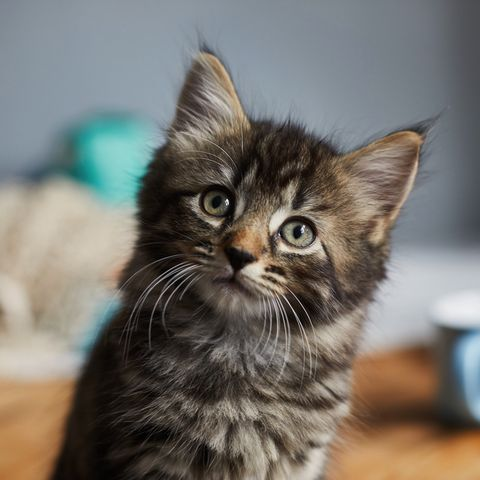
\includegraphics[scale=0.38]{Capitulos/Figuras/gatito.jpg}
	\caption{Un gatito}
	\label{gatito}
\end{figure}

\lipsum[8]

\section{Tema 3} %SIGUIENTE TEMA O CAPITULO DE LA INTRODUCCIÓN
\lipsum[9-10]

%Ejemplo de Pseudocodigo
\begin{algorithm}
    \caption{An algorithm with caption}\label{alg:cap}
    \begin{algorithmic}
        \Require $n \geq 0$
        \Ensure $y = x^n$
        \State $y \gets 1$
        \State $X \gets x$
        \State $N \gets n$
        \While{$N \neq 0$}
        \If{$N$ is even}
            \State $X \gets X \times X$
            \State $N \gets \frac{N}{2}$  \Comment{This is a comment}
        \ElsIf{$N$ is odd}
            \State $y \gets y \times X$
            \State $N \gets N - 1$
        \EndIf
        \EndWhile
    \end{algorithmic}
\end{algorithm}
\lipsum[11-13]

\section{Tema 4} %SIGUIENTE TEMA O CAPITULO DE LA INTRODUCCIÓN
\lipsum[14-16]

%Ejemplo de definición de ecuación
\begin{defn} [\cite{Booker2019Cracking33}] Ecuación de la vida, el universo y todo lo demás resuelta
    $$x^3+y^3+z^3=42$$
    $$(-80538738812075974)^3 + 80435758145817515^3 + 12602123297335631^3 = 42$$
\end{defn}

\lipsum[17-25]
\section{Tema 5} %SIGUIENTE TEMA O CAPITULO DE LA INTRODUCCIÓN
\lipsum[26-28]

%Ejemplo de doble figura
\begin{figure}
\begin{subfigure}{.5\textwidth}
  \centering
  
\includegraphics[width=.8\linewidth]{Capitulos/Figuras/gato_bug.jpg}
  \caption{}
  \label{fig:sfig1}
\end{subfigure}%
\begin{subfigure}{.5\textwidth}
  \centering
  
\includegraphics[width=.8\linewidth]{Capitulos/Figuras/gato_bug_2.jpg}
  \caption{}
  \label{fig:sfig2}
\end{subfigure}
\caption{Gatos bugueadisimos, (a) Gato bug blanco. (b) Gato bug negro.}
\label{fig:fig}
\end{figure}
\lipsum[29-31]

\section{Tema 6} %SIGUIENTE TEMA O CAPITULO DE LA INTRODUCCIÓN
\lipsum[32-35]